% %%%%%%%%%%%%%%%%%%%%%%%%%%%%%%%%%%%%%%%%%%%%%%%%%%%%%%%%%%%%%%%%%%%%%%%%%%%%%
% 选择 isBeamerMode -> 0: 文件,1:幻灯片
% %%%%%%%%%%%%%%%%%%%%%%%%%%%%%%%%%%%%%%%%%%%%%%%%%%%%%%%%%%%%%%%%%%%%%%%%%%%%%
\def\isBeamerMode{1}
\if 0\isBeamerMode
    \makeatletter
    \newif\ifntx@origotf
    \makeatother
    \PassOptionsToPackage{nofontspec}{newtxtext}
    \documentclass[lang=cn]{elegantpaper}
    \usepackage{xcolor}
    \renewenvironment{frame}[1][]{}{}
    \setcounter{tocdepth}{1}
\else
    \documentclass{ctexbeamer}
    \usepackage{listings}
    \usepackage{xcolor}
    \usepackage{multicol}
    \usepackage{indentfirst}
    \setlength{\parindent}{2em}
    % 幻灯片的一些配置
    \usetheme{Berlin}
    \AtBeginSection[] {
        \begin{frame}
            \begin{multicols}{2}
            \tableofcontents[currentsection, hideallsubsections]
            \end{multicols}
        \end{frame}
    }
\fi

\usepackage{booktabs}



% %%%%%%%%%%%%%%%%%%%%%%%%%%%%%%%%%%%%%%%%%%%%%%%%%%%%%%%%%%%%%%%%%%%%%%%%%%%%%
% 一些宏定义和相关配置
% %%%%%%%%%%%%%%%%%%%%%%%%%%%%%%%%%%%%%%%%%%%%%%%%%%%%%%%%%%%%%%%%%%%%%%%%%%%%%
% 让 \normalsizeHeight 为汉字的字宽
\makeatletter
\normalsize
\newlength{\normalsizeHeight}
\setlength{\normalsizeHeight}{\f@size pt}
\makeatother


% \sectionAuthor{<出题人姓名>}
% 用于添加章节作者
\newcommand\sectionAuthor[1]{%
    % style at begin
    \if 0\isBeamerMode\relax%
        \small\color{gray}%
        \vspace*{-1cm}\hfill%
    \else%
        \vspace*{0.3cm}%
    \fi%
    % text...
    \noindent Tutorial by \textbf{#1}.%
    \if 1\isBeamerMode\relax%
        \par%
    \fi%
    % style at end
    \if 0\isBeamerMode\relax%
        \normalsize\color{black}%
        \vspace*{0.3cm}%
    \else%
        \vspace*{0.5cm}%
    \fi}


% \addCode{<章节名>}{<代码文件名>}{<高亮名>}
% e.g. \addCode{小明和他的朋友}{xiaomi_and_his_friend.cpp}{cpp}
% 用于陈列代码
\newcommand\addCode[3]{%
    \subsection{#1}%
    \lstinputlisting[language=#3]{#2}}


% \cmd{<代码>}
% 用于陈列行内代码
\newcommand\cmd[1]{%
    \texttt{#1}}


% 配置陈列代码的风格
\lstset{
    xleftmargin         =   2\normalsizeHeight, % 缩进
    basicstyle          =   \ttfamily,          % 基本代码风格
    keywordstyle        =   \bfseries,          % 关键字风格
    commentstyle        =   \rmfamily\itshape,  % 注释的风格,斜体
    stringstyle         =   \ttfamily,          % 字符串风格
    flexiblecolumns,                            % 别问为什么,加上这个
    numbers             =   left,               % 行号的位置在左边
    showspaces          =   false,              % 是否显示空格,显示了有点乱,所以不现实了
    numberstyle         =   \ttfamily,          % 行号的样式,小五号,tt等宽字体
    showstringspaces    =   false,
    captionpos          =   t,                  % 这段代码的名字所呈现的位置,t指的是top上面
    frame               =   lrtb,               % 显示边框
    columns             =   fixed,              % 字的宽度固定
    basewidth           =   0.5em,              % 固定为 0.5em
    tabsize             =   4,                  % tab 展示为 4 个空格宽度
    keywordstyle        =   \color{blue},
    keywordstyle        =   [2] \color{teal},
    stringstyle         =   \color{magenta},
    commentstyle        =   \color{red}\ttfamily,
}



% %%%%%%%%%%%%%%%%%%%%%%%%%%%%%%%%%%%%%%%%%%%%%%%%%%%%%%%%%%%%%%%%%%%%%%%%%%%%%
% 在这里编辑基础信息
% %%%%%%%%%%%%%%%%%%%%%%%%%%%%%%%%%%%%%%%%%%%%%%%%%%%%%%%%%%%%%%%%%%%%%%%%%%%%%
\title{寒假集训 - 字符串和数论}
\author{苏州大学 ACM 集训队}



\begin{document}

% %%%%%%%%%%%%%%%%%%%%%%%%%%%%%%%%%%%%%%%%%%%%%%%%%%%%%%%%%%%%%%%%%%%%%%%%%%%%%
% 生成标题
% %%%%%%%%%%%%%%%%%%%%%%%%%%%%%%%%%%%%%%%%%%%%%%%%%%%%%%%%%%%%%%%%%%%%%%%%%%%%%
% 如果它是 paper
\if 0\isBeamerMode\relax
    \maketitle
    \tableofcontents
    \newpage
\fi

% 如果它是 beamer
\if 1\isBeamerMode\relax
    \frame{\titlepage}
\fi



% %%%%%%%%%%%%%%%%%%%%%%%%%%%%%%%%%%%%%%%%%%%%%%%%%%%%%%%%%%%%%%%%%%%%%%%%%%%%%
% 在这里 include 所有题解
% %%%%%%%%%%%%%%%%%%%%%%%%%%%%%%%%%%%%%%%%%%%%%%%%%%%%%%%%%%%%%%%%%%%%%%%%%%%%%
\def\TOCName{字符串基础} 
% %%%%%%%%%%%%%%%%%%%%%%%%%%%%%%%%%%%%%%%%%%%%%%%%%%%%%%%%%%%%%%%%%%%%%%%%%%%%%
% 在这里填入题目
% %%%%%%%%%%%%%%%%%%%%%%%%%%%%%%%%%%%%%%%%%%%%%%%%%%%%%%%%%%%%%%%%%%%%%%%%%%%%%
\def\sectionName{字符串 - 基础字符串知识}



% 如果它是 beamer
\if 1\isBeamerMode\relax
    \section[\TOCName]{\sectionName}
\fi
% 如果它是 paper
\if 0\isBeamerMode\relax
    \section[\TOCName\ -\ \sectionName]{\sectionName}
\fi

\begin{frame}

% 如果它是 beamer
\if 1\isBeamerMode\relax
    \noindent {\Huge \sectionName}\par
\fi

% %%%%%%%%%%%%%%%%%%%%%%%%%%%%%%%%%%%%%%%%%%%%%%%%%%%%%%%%%%%%%%%%%%%%%%%%%%%%%
% 在这里填入你的名字
% %%%%%%%%%%%%%%%%%%%%%%%%%%%%%%%%%%%%%%%%%%%%%%%%%%%%%%%%%%%%%%%%%%%%%%%%%%%%%
\sectionAuthor{Ding Yuyang}



% %%%%%%%%%%%%%%%%%%%%%%%%%%%%%%%%%%%%%%%%%%%%%%%%%%%%%%%%%%%%%%%%%%%%%%%%%%%%%
% 这里可以写感想(嘲讽,bushi),也可以不写!!!
% %%%%%%%%%%%%%%%%%%%%%%%%%%%%%%%%%%%%%%%%%%%%%%%%%%%%%%%%%%%%%%%%%%%%%%%%%%%%%



\end{frame}

% %%%%%%%%%%%%%%%%%%%%%%%%%%%%%%%%%%%%%%%%%%%%%%%%%%%%%%%%%%%%%%%%%%%%%%%%%%%%%
% 这里开始写简单的题目意思 ~
% %%%%%%%%%%%%%%%%%%%%%%%%%%%%%%%%%%%%%%%%%%%%%%%%%%%%%%%%%%%%%%%%%%%%%%%%%%%%%
\subsection{C/C++ 字符串基本知识}
\begin{frame}{char 类型} % 如果一个 frame 写不下的话,多开几个就好了~
\begin{itemize}
    \item \cmd{char ch='a';} 实际上存储的是字符的 ascii 码。
    \item \cmd{'a' + 3} 注意单引号和双引号不同。
\end{itemize}
\end{frame}

\begin{frame}{C 风格字符串}
\begin{itemize}
    \item 字符数组。
    \item \cmd{char s[6] = "abcde";}
\end{itemize}
\end{frame}

\begin{frame}{字符串结束符}
\begin{itemize}
    \item 末尾添加 \cmd{'\textbackslash 0'} 表示字符串结束。
    \item \texttt{char s[6] = "Hello";}
    \item \texttt{char s[6] = \{'H', 'e', 'l', 'l', 'o', '\textbackslash 0'\};}
    \item \texttt{char s[6] = \{'H', 'e', 'l', 'l', 'o'\};}
    \item \texttt{char s[] = "Hello";}
\end{itemize}
\end{frame}

\begin{frame}{字符串读入}
\begin{itemize}
    \item \texttt{s[0]} 是首个字符。
    \item \texttt{scanf("\%s", s)}。
    \item \texttt{scanf("\%s", \&s[0])}。
    \item \texttt{cin >> s}。
\end{itemize}

\begin{itemize}
    \item \texttt{s[1]} 是首个字符。
    \item \texttt{scanf("\%s", s + 1)}。
    \item \texttt{scanf("\%s", \&s[1])}。
    \item \texttt{cin >> s + 1}。
\end{itemize}
\end{frame}

\begin{frame}{整行读入}
\begin{itemize}
    \item \texttt{gets(str)}。
    \item \texttt{getline(cin, str)},这里 \cmd{str} 的类型应该是 \cmd{string}。
    \item \texttt{fgets(str, N, stdin)}。
\end{itemize}
\end{frame}

\begin{frame}{字符串函数}
\begin{itemize}
    \item \texttt{strlen(s)}。
    \item 返回从 \cmd{s} 下标 $0$ 开始的字符串长度(不包括 \cmd{'\textbackslash
        0'})。
    \item 复杂度为 $O(|S|)$。
    \item 如果下标从 $1$ 开始的话,则使用 \texttt{strlen(s + 1)}。
\end{itemize}
\end{frame}

\begin{frame}[fragile]{一个常见的错误}
\begin{lstlisting}[language=C++]
for (int i = 0; i < strlen(s); i++) {
    // ......
}
\end{lstlisting}

时间复杂度不是 $O(|S|)$ 而是 $O(|S|^2)$。
\end{frame}

\begin{frame}{字符串函数}
\begin{itemize}
    \item \texttt{strcpy(str1, str2)},用于复制。
    \item \texttt{strcmp(str1, str2)},用于比较。
\end{itemize}
\end{frame}

\begin{frame}{string 读入}
\begin{itemize}
    \item \texttt{cin >> s},字符串输入。
    \item \texttt{cout << s},字符串输出。
    \item \texttt{s.size()},时间复杂度: $O(1)$。
\end{itemize}
\end{frame}

\def\TOCName{字典树} 
% %%%%%%%%%%%%%%%%%%%%%%%%%%%%%%%%%%%%%%%%%%%%%%%%%%%%%%%%%%%%%%%%%%%%%%%%%%%%%
% 在这里填入题目
% %%%%%%%%%%%%%%%%%%%%%%%%%%%%%%%%%%%%%%%%%%%%%%%%%%%%%%%%%%%%%%%%%%%%%%%%%%%%%
\def\sectionName{字符串 - 字典树}



% 如果它是 beamer
\if 1\isBeamerMode\relax
    \section[\TOCName]{\sectionName}
\fi
% 如果它是 paper
\if 0\isBeamerMode\relax
    \section[\TOCName\ -\ \sectionName]{\sectionName}
\fi

\begin{frame}

% 如果它是 beamer
\if 1\isBeamerMode\relax
    \noindent {\Huge \sectionName}\par
\fi

% %%%%%%%%%%%%%%%%%%%%%%%%%%%%%%%%%%%%%%%%%%%%%%%%%%%%%%%%%%%%%%%%%%%%%%%%%%%%%
% 在这里填入你的名字
% %%%%%%%%%%%%%%%%%%%%%%%%%%%%%%%%%%%%%%%%%%%%%%%%%%%%%%%%%%%%%%%%%%%%%%%%%%%%%
\sectionAuthor{Ding Yuyang}



% %%%%%%%%%%%%%%%%%%%%%%%%%%%%%%%%%%%%%%%%%%%%%%%%%%%%%%%%%%%%%%%%%%%%%%%%%%%%%
% 这里可以写感想(嘲讽,bushi),也可以不写!!!
% %%%%%%%%%%%%%%%%%%%%%%%%%%%%%%%%%%%%%%%%%%%%%%%%%%%%%%%%%%%%%%%%%%%%%%%%%%%%%
\noindent 字典树是字符串算法中比较基础的算法之一。



\end{frame}

% %%%%%%%%%%%%%%%%%%%%%%%%%%%%%%%%%%%%%%%%%%%%%%%%%%%%%%%%%%%%%%%%%%%%%%%%%%%%%
% 这里开始写简单的题目意思 ~
% %%%%%%%%%%%%%%%%%%%%%%%%%%%%%%%%%%%%%%%%%%%%%%%%%%%%%%%%%%%%%%%%%%%%%%%%%%%%%
\subsection{字典树状态}
\begin{frame}{字典树的形态举例} % 如果一个 frame 写不下的话,多开几个就好了~
比如含有 and, as, at, cn, com 的字典树:
\begin{center}
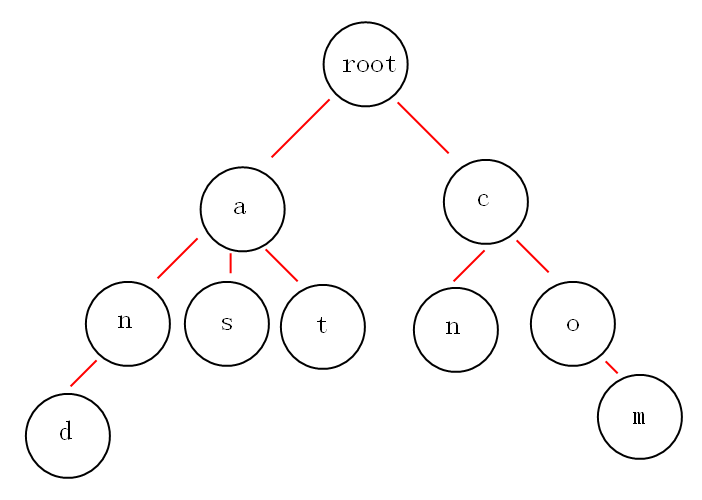
\includegraphics[width=0.7\textwidth]{./pic/trie_state.png}
\end{center}
\end{frame}

\begin{frame}
\begin{itemize}
    \item 根节点不包含字符,除根节点外的每一个子节点都包含一个字符。
    \item 从根节点到某一节点,路径上经过的字符连接起来,就是该节点对应的字符串。
    \item 每个单词的前缀作为一个字符节点保存。
\end{itemize}
\end{frame}

\begin{frame}[fragile]{新建节点}
时间复杂度: $O(|\sum|)$, 其中 $\sum$ 是字符集。

\begin{lstlisting}[language=C++]
int newnode(void) {
    ++num;
    color[num] = 0;
    cnt[num] = 0;
    memset(tree[num], 0, sizeof(tree[num]));
    return num;
}
\end{lstlisting}
\end{frame}

\begin{frame}[fragile]{字典树的插入操作}
\begin{lstlisting}[language=C++]
void insert(char s[]) {
    int n = strlen(s), p = 0;
    for (int i = 0; i < n; i++){
        int c = s[i] - 'a';
        if (tree[p][c] == 0) tree[p][c] = newnode();
        p = tree[p][c];
        cnt[p]++;
    }
    color[p]++;
}
\end{lstlisting}
\end{frame}

\begin{frame}[fragile]{字典树的查找操作}
\begin{lstlisting}[language=C++]
int find(char s[]) {
    int n = strlen(s), p = 0;
    for (int i = 0; i < n; i++){
        int c = s[i] - 'a';
        if (tree[p][c] == 0) return 0;
        p = tree[p][c];
    }
    return color[p];
}
\end{lstlisting}
\end{frame}

\subsection{做题}
\begin{frame}{做题}
TODO。
% \begin{itemize}
%     \item HDU - 1251。
% \end{itemize}
% \end{frame}
% 
% \begin{frame}
% \begin{itemize}
%     \item 给定一个 $n$ 个数的数组 $a$, 满足 $1\leq n\leq 10^5, 0\leq a_i\leq
%         10^9$。
%     \item 现在询问 $m$ 次,每次给出一个数 $x$, 数组中与 $x$ 异或值最大的数是多少。
%         $1\leq m\leq 10^5$。
% \end{itemize}
% \end{frame}
% 
% \begin{frame}
% \begin{itemize}
%     \item 暴力复杂度: $O(nm)$
%     \item 怎么用字典树?
% \end{itemize}
% \end{frame}
% 
% \begin{frame}
% \begin{center}
% 01trie + 贪心
% \end{center}
% \end{frame}
% 
% \begin{frame}
% \begin{itemize}
%     \item 提高难度
%     \item 对于 $n$ 个数的数组,球最大区间异或和
%     \item 区间 $(l, r)$ 的区间异或和为 $a[l]\oplus a[l + 1]\oplus ...\oplus a[r]$
% \end{itemize}
\end{frame}


\def\TOCName{位运算} 
% %%%%%%%%%%%%%%%%%%%%%%%%%%%%%%%%%%%%%%%%%%%%%%%%%%%%%%%%%%%%%%%%%%%%%%%%%%%%%
% 在这里填入题目
% %%%%%%%%%%%%%%%%%%%%%%%%%%%%%%%%%%%%%%%%%%%%%%%%%%%%%%%%%%%%%%%%%%%%%%%%%%%%%
\def\sectionName{数论 - 位运算}



% 如果它是 beamer
\if 1\isBeamerMode\relax
    \section[\TOCName]{\sectionName}
\fi
% 如果它是 paper
\if 0\isBeamerMode\relax
    \section[\TOCName\ -\ \sectionName]{\sectionName}
\fi

\begin{frame}

% 如果它是 beamer
\if 1\isBeamerMode\relax
    {\Huge \sectionName}\par
\fi

% %%%%%%%%%%%%%%%%%%%%%%%%%%%%%%%%%%%%%%%%%%%%%%%%%%%%%%%%%%%%%%%%%%%%%%%%%%%%%
% 在这里填入你的名字
% %%%%%%%%%%%%%%%%%%%%%%%%%%%%%%%%%%%%%%%%%%%%%%%%%%%%%%%%%%%%%%%%%%%%%%%%%%%%%
\sectionAuthor{Peterlits Zo}



% %%%%%%%%%%%%%%%%%%%%%%%%%%%%%%%%%%%%%%%%%%%%%%%%%%%%%%%%%%%%%%%%%%%%%%%%%%%%%
% 这里可以写感想(嘲讽,bushi),也可以不写!!!
% %%%%%%%%%%%%%%%%%%%%%%%%%%%%%%%%%%%%%%%%%%%%%%%%%%%%%%%%%%%%%%%%%%%%%%%%%%%%%
位运算很巧妙的~



\end{frame}

% %%%%%%%%%%%%%%%%%%%%%%%%%%%%%%%%%%%%%%%%%%%%%%%%%%%%%%%%%%%%%%%%%%%%%%%%%%%%%
% 逻辑代数
% %%%%%%%%%%%%%%%%%%%%%%%%%%%%%%%%%%%%%%%%%%%%%%%%%%%%%%%%%%%%%%%%%%%%%%%%%%%%%
\subsection{逻辑代数}
\begin{frame} % 如果一个 frame 写不下的话,多开几个就好了~
逻辑代数中只有两个元素,既真和假。举例来说的话,我们有:
\begin{itemize}
    \item 太阳从东边升起。\pause $\to T$。
    \item $1 + 1 = 3$。\pause $\to F$。
\end{itemize}

可以看到命题可以得到它的真值。接下来我们要定义它们的运算。
\end{frame}

\begin{frame}
一般而言我们有四个运算:
\begin{itemize}
    \item 或。两个中有至少一个为真它就是真。我们定义符号有 $\lor$。\pause
    \item 与。两个中同时为真它才是真。我们定义符号有 $\land$。\pause
    \item 非。它能把真的变成假的,把假的变成真的。我们定义符号有 $\lnot$。\pause
    \item 亦或。两个中\textbf{有且仅有}一个为真它才是真。我们定义符号有 $\oplus$。
\end{itemize}
\end{frame}

\begin{frame}
\begin{block}{符号表}
或:$\lor$\hfill 与:$\land$\hfill 非:$\lnot$\hfill 亦或:$\oplus$ \hfill
\end{block}

用抽象后的逻辑代数可以帮助我们更好的理解和运算。

比如:如果太阳从东边升起,或者,太阳从西边升起并且 $1 + 1 = 3$ 的时候,Peterlits
就会摆烂。我们希望得知 Peterlits 到底会不会摆烂。那么它对应的表达式就是:\pause

\[T \lor (F \land F)\]

运算可得,其结果是 $T$。
\end{frame}

\begin{frame}
\begin{block}{符号表}
或:$\lor$\hfill 与:$\land$\hfill 非:$\lnot$\hfill 亦或:$\oplus$ \hfill
\end{block}

因为在 ASCII 下不太好输入,C++ 用以下的符号来代表逻辑代数的运算:
\begin{itemize}
    \item 或。\cmd{||}。\pause
    \item 与。\cmd{\&\&}。\pause
    \item 非。\cmd{!}。\pause
    \item 亦或。嘻嘻,C++ 没有这个。
\end{itemize}
\end{frame}

\begin{frame}[fragile]
\begin{block}{符号表}
或:$\lor$ / \cmd{||}\hfill
与:$\land$ / \cmd{\&\&}\hfill
非:$\lnot$ / \cmd{!}\hfill
亦或:$\oplus$ \hfill
\end{block}

\begin{lstlisting}[language=C++]
int foo = 10;
int bar = 30;

if (foo < bar || false) {
    printf("ooooops!!"); // 这个一定会输出的!
}
\end{lstlisting}
\end{frame}

\begin{frame}[fragile]
在 C++ 中,我们认为,一切非零的都是真的($T$),而零是假的($F$)。\pause

也就是说下面的我们会得到输出 \cmd{1}:
\begin{lstlisting}[language=C++]
// 不过用数字来做逻辑运算太少见,所以应该会 WARNING。
printf("%d", (100 || 0));
\end{lstlisting}
\end{frame}

\begin{frame}
那么位运算就是我们上面讲的吗?不是~不过有一些关系的。
\end{frame}


% %%%%%%%%%%%%%%%%%%%%%%%%%%%%%%%%%%%%%%%%%%%%%%%%%%%%%%%%%%%%%%%%%%%%%%%%%%%%%
% 位运算
% %%%%%%%%%%%%%%%%%%%%%%%%%%%%%%%%%%%%%%%%%%%%%%%%%%%%%%%%%%%%%%%%%%%%%%%%%%%%%
\subsection{位运算}
\begin{frame}
\begin{block}{符号表}
或:$\lor$ / \cmd{||}\hfill
与:$\land$ / \cmd{\&\&}\hfill
非:$\lnot$ / \cmd{!}\hfill
亦或:$\oplus$ \hfill
\end{block}
我们知道,计算机内的一些东西都是二进制的,无论是数字、字符还是字符串,都是二进制
的。如果能把二进制映射到 $T/F$ 上就好了:\pause
\begin{itemize}
    \item $1 \to T$。\pause
    \item $0 \to F$。\pause
\end{itemize}

根据这个,我们自然而然的就得到了位运算了:数值都是由 $0 / 1$ 组成的,那么我们让
对应的值进行逻辑运算,一一收集起来就可以得到结果了。
\end{frame}

\begin{frame}
\begin{block}{符号表}
或:$\lor$ / \cmd{||}\hfill
与:$\land$ / \cmd{\&\&}\hfill
非:$\lnot$ / \cmd{!}\hfill
亦或:$\oplus$ \hfill
\end{block}

我们定义位运算如下:
\begin{itemize}
    \item 按位与。\cmd{\&}。
    \item 按位或。\cmd{|}。
    \item 按位取反。\cmd{\ \~}。
    \item 按位亦或。\cmd{\ \^}。
\end{itemize}

有的时候,我们说某些操作的时候,可能会省略掉\textbf{按位}两个字,这种时候就需要
自己判断到底说的是逻辑运算还是位运算了。
\end{frame}

\begin{frame}[fragile]
\begin{block}{符号表}
或:$\lor$ / \cmd{||} / \cmd{|}(按位)\hfill
与:$\land$ / \cmd{\&\&} / \cmd{\&}(按位)\hfill

非:$\lnot$ / \cmd{!} / \cmd{\ \~}(按位)\hfill
亦或:$\oplus$ / \cmd{\ \^}(按位) \hfill
\end{block}

比如说我们可以来模拟一哈按位亦或。我们知道,亦或的结果为真,当且仅当一个为真。

也就是说,我们有:
\begin{lstlisting}[language=C++]
int a = 0 ^ 0; \\ a = 0,因为只有 0 个 1。
int b = 0 ^ 1; \\ b = 1,因为正好有 1 个 1。
int c = 1 ^ 0; \\ c = 1,因为正好有 1 个 1。
int d = 1 ^ 1; \\ c = 2,因为有 2 个 1。
\end{lstlisting}
\end{frame}

\begin{frame}
现在我们希望得到(下列数字均在表示在二进制下)下述表达式的运算结果:\[
    1000100101110 \text{\cmd{\ \^}} 1010100011010
\] \pause

那么有:
\begin{center}
\begin{tabular}{lrrrrrrrrrrrrr}
    \toprule
    $a$  & $1$ & $0$ & $0$ & $0$ & $1$ & $0$ & $0$ & $1$ & $0$ & $1$ & $1$ & $1$ & $0$ \\
    $b$  & $1$ & $0$ & $1$ & $0$ & $1$ & $0$ & $0$ & $0$ & $1$ & $1$ & $0$ & $1$ & $0$ \\
    \midrule
    结果 & $0$ & $0$ & $1$ & $0$ & $0$ & $0$ & $0$ & $1$ & $1$ & $0$ & $1$ & $0$ & $0$ \\
    \bottomrule
\end{tabular}
\end{center}
\end{frame}

\begin{frame}
\begin{block}{符号表}
或:$\lor$ / \cmd{||} / \cmd{|}(按位)\hfill
与:$\land$ / \cmd{\&\&} / \cmd{\&}(按位)\hfill

非:$\lnot$ / \cmd{!} / \cmd{\ \~}(按位)\hfill
亦或:$\oplus$ / \cmd{\ \^}(按位) \hfill
\end{block}

除了符号表里的东西,我们还有其他的运算符:\cmd{>>} 和 \cmd{<<}。

它可以让一个数在二进制下左移或者右移。
\end{frame}

\begin{frame}
我们注意到,一个数一旦左移一位的话,随之带来的就是这个数会变大为原来的两倍。那么
我们就可以用 \cmd{1 << n} 来表示 $2^n$\footnote{这里和下面的东西,均假设我们的被
操作数是一个正数}。

同理,我们可以用右移来表示除以 $2$ 并向下取整。
\end{frame}

\begin{frame}
我们发现了一个数是偶数,当且仅当二进制下最后一个位为 $0$,那么我们要是能够把这玩
意取出来就好了。\pause

我们可以使用 \cmd{a \& 1} 这个位运算。
\end{frame}

\begin{frame}
当然位运算的一些小技巧还有很多都没见。不过讲快速幂肯定是绰绰有余了。
\end{frame}

\def\TOCName{模运算} 
% %%%%%%%%%%%%%%%%%%%%%%%%%%%%%%%%%%%%%%%%%%%%%%%%%%%%%%%%%%%%%%%%%%%%%%%%%%%%%
% 在这里填入题目
% %%%%%%%%%%%%%%%%%%%%%%%%%%%%%%%%%%%%%%%%%%%%%%%%%%%%%%%%%%%%%%%%%%%%%%%%%%%%%
\def\sectionName{数论 - 模运算}



% 如果它是 beamer
\if 1\isBeamerMode\relax
    \section[\TOCName]{\sectionName}
\fi
% 如果它是 paper
\if 0\isBeamerMode\relax
    \section[\TOCName\ -\ \sectionName]{\sectionName}
\fi

\begin{frame}

% 如果它是 beamer
\if 1\isBeamerMode\relax
    \noindent{\Huge \sectionName}\par
\fi

% %%%%%%%%%%%%%%%%%%%%%%%%%%%%%%%%%%%%%%%%%%%%%%%%%%%%%%%%%%%%%%%%%%%%%%%%%%%%%
% 在这里填入你的名字
% %%%%%%%%%%%%%%%%%%%%%%%%%%%%%%%%%%%%%%%%%%%%%%%%%%%%%%%%%%%%%%%%%%%%%%%%%%%%%
\sectionAuthor{Peterlits Zo}



% %%%%%%%%%%%%%%%%%%%%%%%%%%%%%%%%%%%%%%%%%%%%%%%%%%%%%%%%%%%%%%%%%%%%%%%%%%%%%
% 这里可以写感想(嘲讽,bushi),也可以不写!!!
% %%%%%%%%%%%%%%%%%%%%%%%%%%%%%%%%%%%%%%%%%%%%%%%%%%%%%%%%%%%%%%%%%%%%%%%%%%%%%
\noindent 模运算,模来模去!



\end{frame}

% %%%%%%%%%%%%%%%%%%%%%%%%%%%%%%%%%%%%%%%%%%%%%%%%%%%%%%%%%%%%%%%%%%%%%%%%%%%%%
% 取模
% %%%%%%%%%%%%%%%%%%%%%%%%%%%%%%%%%%%%%%%%%%%%%%%%%%%%%%%%%%%%%%%%%%%%%%%%%%%%%
\subsection{取模}

\begin{frame}
首先我们来定义一哈取模:对于数 $a$ 和 $b$ 而言,我们找到 $a$ 除以 $b$ 之后的余数,
那就是取模啦!真简单。其中,我们把运算符定义为 $\bmod$。\pause

举例子来说明:
\begin{itemize}
    \item $5 \bmod 4 = 1$。\pause
    \item $100 \bmod 5 = 0$。\pause
    \item $5 \bmod 3 = 2$。
\end{itemize}

在 C++ 下,我们用符号 \cmd{\%} 来表示取余。
\end{frame}

\begin{frame}
我们定义完了取余,接下来我们就定义一哈同余。假设模数是 $m$(mod 的首字母~),而
有两个数 $a$ 和 $b$,如果满足:\[
    a \bmod m = b \bmod m
\]\pause
那么我们就说在模 $m$ 下,$a$ 和 $b$ \textbf{同余}。

我们记为:\[
    a \equiv b \pmod m
\]
\end{frame}

\begin{frame}
可以注意到一个很小的性质,那就是,对于任意一个数 $n$ 而言,都存在一个整数 $i \in
[0, m - 1]$,使得 $n$ 和 $i$ 同余。

还有一个性质,那就是 $a$ 和 $b$ 同余,当且仅当 $a - b \equiv 0 \pmod m$。
\end{frame}

\subsection{模运算的性质}

\begin{frame}
我们现在需要深入研究一哈模运算的性质。

首先是:\[
    a + b \equiv (a \bmod m) + (b \bmod m) \pmod m
\] \pause

为了证明这个,我们不妨假设 $a' = a \bmod m$,同理有 $b'$。那么 $a = a' + p_a m$,
同理 $b = b' + p_b m$。

那么代入有:\[
    a' + p_a m + b' + p_b m = a' + b' + (p_a + p_b) m
\]

那么左边减右边,得到 $(p_a + p_b) m$,这个很明显在模 $m$ 下和 $0$ 同余嘛。
\end{frame}

\begin{frame}[fragile]
同理对于减法也是这样的。不过说道减法,一般而言,C++ 的 \cmd{\%} 取模运算符并不能
让负数也能得到在 $[0, m - 1]$ 部分的模。这是因为在 C++ 中有:
\begin{lstlisting}[language=C++]
(-a) % b = -(a % b)
\end{lstlisting}\pause
所以说,一般而言,我们会使用下面的东西来得到对应的值:
\begin{lstlisting}[language=C++]
(a % b + b) % b
\end{lstlisting}
\end{frame}

\begin{frame}
同理我们有:\[
    a \times b \equiv (a \bmod m) \times (b \bmod m) \pmod m
\] \pause

证明方法和证明加法很像。这里就略去证明了。
\end{frame}

\begin{frame}
那么除法呢?这个不太好讲,我们可以留到后面讲逆元的时候再讲。但是现在我们需要知道
的是,对于除法而言,下面的式子是不成立的:\[
    a / b \equiv (a \bmod m) / (b \bmod m) \pmod m
\]

比如说,$a = 6$,$b = 3$,而 $m = 5$。更何况,我们难过地发现,除法带来了小数。而
后面我们可以通过学逆元惊喜地发现,我们可以让除法搞不出小数来。
\end{frame}

\def\TOCName{快速幂} 
% %%%%%%%%%%%%%%%%%%%%%%%%%%%%%%%%%%%%%%%%%%%%%%%%%%%%%%%%%%%%%%%%%%%%%%%%%%%%%
% 在这里填入题目
% %%%%%%%%%%%%%%%%%%%%%%%%%%%%%%%%%%%%%%%%%%%%%%%%%%%%%%%%%%%%%%%%%%%%%%%%%%%%%
\def\sectionName{数论 - 快速幂}



% 如果它是 beamer
\if 1\isBeamerMode\relax
    \section[\TOCName]{\sectionName}
\fi
% 如果它是 paper
\if 0\isBeamerMode\relax
    \section[\TOCName\ -\ \sectionName]{\sectionName}
\fi

\begin{frame}

% 如果它是 beamer
\if 1\isBeamerMode\relax
    \noindent{\Huge \sectionName}\par
\fi

% %%%%%%%%%%%%%%%%%%%%%%%%%%%%%%%%%%%%%%%%%%%%%%%%%%%%%%%%%%%%%%%%%%%%%%%%%%%%%
% 在这里填入你的名字
% %%%%%%%%%%%%%%%%%%%%%%%%%%%%%%%%%%%%%%%%%%%%%%%%%%%%%%%%%%%%%%%%%%%%%%%%%%%%%
\sectionAuthor{Peterlits Zo}



% %%%%%%%%%%%%%%%%%%%%%%%%%%%%%%%%%%%%%%%%%%%%%%%%%%%%%%%%%%%%%%%%%%%%%%%%%%%%%
% 这里可以写感想(嘲讽,bushi),也可以不写!!!
% %%%%%%%%%%%%%%%%%%%%%%%%%%%%%%%%%%%%%%%%%%%%%%%%%%%%%%%%%%%%%%%%%%%%%%%%%%%%%
\noindent 快速幂,xiuxiuxiu~



\end{frame}

% %%%%%%%%%%%%%%%%%%%%%%%%%%%%%%%%%%%%%%%%%%%%%%%%%%%%%%%%%%%%%%%%%%%%%%%%%%%%%
% 逻辑代数
% %%%%%%%%%%%%%%%%%%%%%%%%%%%%%%%%%%%%%%%%%%%%%%%%%%%%%%%%%%%%%%%%%%%%%%%%%%%%%
\begin{frame}
\end{frame}

\def\TOCName{BSGS} 
% %%%%%%%%%%%%%%%%%%%%%%%%%%%%%%%%%%%%%%%%%%%%%%%%%%%%%%%%%%%%%%%%%%%%%%%%%%%%%
% 在这里填入题目
% %%%%%%%%%%%%%%%%%%%%%%%%%%%%%%%%%%%%%%%%%%%%%%%%%%%%%%%%%%%%%%%%%%%%%%%%%%%%%
\def\sectionName{数论 - BSGS}



% 如果它是 beamer
\if 1\isBeamerMode\relax
    \section[\TOCName]{\sectionName}
\fi
% 如果它是 paper
\if 0\isBeamerMode\relax
    \section[\TOCName\ -\ \sectionName]{\sectionName}
\fi

\begin{frame}

% 如果它是 beamer
\if 1\isBeamerMode\relax
    \noindent{\Huge \sectionName}\par
\fi

% %%%%%%%%%%%%%%%%%%%%%%%%%%%%%%%%%%%%%%%%%%%%%%%%%%%%%%%%%%%%%%%%%%%%%%%%%%%%%
% 在这里填入你的名字
% %%%%%%%%%%%%%%%%%%%%%%%%%%%%%%%%%%%%%%%%%%%%%%%%%%%%%%%%%%%%%%%%%%%%%%%%%%%%%
\sectionAuthor{Peterlits Zo}



% %%%%%%%%%%%%%%%%%%%%%%%%%%%%%%%%%%%%%%%%%%%%%%%%%%%%%%%%%%%%%%%%%%%%%%%%%%%%%
% 这里可以写感想(嘲讽,bushi),也可以不写!!!
% %%%%%%%%%%%%%%%%%%%%%%%%%%%%%%%%%%%%%%%%%%%%%%%%%%%%%%%%%%%%%%%%%%%%%%%%%%%%%
\noindent 用在区间里会很快哦。



\end{frame}

% %%%%%%%%%%%%%%%%%%%%%%%%%%%%%%%%%%%%%%%%%%%%%%%%%%%%%%%%%%%%%%%%%%%%%%%%%%%%%
% 取模
% %%%%%%%%%%%%%%%%%%%%%%%%%%%%%%%%%%%%%%%%%%%%%%%%%%%%%%%%%%%%%%%%%%%%%%%%%%%%%
\subsection{取模}

\begin{frame}
我们在快速幂中讲到了,对于 $a^b$ 这种幂运算而言,我们可以在 $O(\lg b)$ 的时间复
杂度内解得结果。

但是有一些题目要求我们能在 $O(1)$ 的时间复杂度来得到。这可不简单哇。
\end{frame}

\begin{frame}
朴素的思想是打表。假设我们的 $b$ 的上限是 $M$,那么我们只要在 $O(M)$ 的时间复杂
度内求得 $i \in [1, M]$ 的 $a^i$ 对应值。\pause

那么我们要求 $a^b$ 直接在表中拿第 $i$ 个就行!!
\end{frame}

\begin{frame}
这种方法的确不错。但是如果 $M$ 太大了就没啥用了。

我们不妨这么想,对于任意一个数 $a^b$ 而言,我们都有,存在 $c$ 和 $d$,使得:$a^b
= a^{c \sqrt M + d}$,其中 $0 \le c < \sqrt M$,而 $0 \le d < \sqrt M$。\pause

那么我们只需要打表 $a^{c \sqrt M}, 0 \le c < \sqrt M$,和 $a^{d}, 0 \le d <
\sqrt M$,我们先算出来 $c$ 和 $d$,再查两次表即可。\pause

可以看到,搞表只要 $O(\sqrt M)$ 的时间/空间复杂度。而我们得到它也是 $O(1)$ 的时
间。
\end{frame}

\begin{frame}
BSGS 的意思是 baby step giant step。这也就是说,我们先 $\sqrt M$ 地移动,移动完
了之后再 $1$ 地移动,即可。
\end{frame}

\begin{frame}
举例子,我们要求 $a^5$ 和 $a^{18}$ 和 $a^{24}$,可以看到我们可以取 $M = 25$,那
么有 $\sqrt M = 5$,令 $a = 2$。\pause

那么有:
\begin{center}
\begin{tabular}{lrrrrr}
    \toprule
    $i$               & $0$ & $1$  & $2$    & $3$     & $4$       \\
    \midrule
    $a^{i \sqrt M}$   & $1$ & $32$ & $1024$ & $32768$ & $1048576$ \\
    $a^{i}$           & $1$ & $2$  & $4$    & $8$     & $16$      \\
    \bottomrule
\end{tabular}
\end{center} \pause

同时,我们有:\pause
\begin{itemize}
    \item $a^5 = a^{1 \times 5 + 0} = a^{1 \sqrt M} \times a^{0} = 32$。\pause
    \item $a^{18} = a^{3 \times 5 + 3} = a^{3 \sqrt M} \times a^{3}$。\pause
    \item $a^{24} = a^{4 \times 5 + 4} = a^{4 \sqrt M} \times a^{4}$。
\end{itemize}
\end{frame}

\begin{frame}
有几个题目:
\begin{itemize}
    \item LiberOJ - p162。
    \item Luogu - P1226。
\end{itemize}
\end{frame}




% %%%%%%%%%%%%%%%%%%%%%%%%%%%%%%%%%%%%%%%%%%%%%%%%%%%%%%%%%%%%%%%%%%%%%%%%%%%%%
% 在这里 include 所有参考代码
% %%%%%%%%%%%%%%%%%%%%%%%%%%%%%%%%%%%%%%%%%%%%%%%%%%%%%%%%%%%%%%%%%%%%%%%%%%%%%
% 如果它是 paper
\if 0\isBeamerMode\relax
\fi



\end{document}
